\subsubsection{Pion Background}\label{section:star_background_pion}
The pion spectra are corrected for weak decays (mainly of $K^0_S$ and $\Lambda^0$), muon contribution and background from the   detector dead-material interactions. The pion decay muons can be identified as pions due to the similar masses. These contributions are obtained from PYTHIA~8 \ac{SD}. Figure~\ref{fig:bkg_pion} shows the background contribution to the pion spectra as a function of $p_\textrm{T}$ in three ranges of $\xi$, separately for $\pi^-$ and $\pi^+$.  Since there were   negligible differences  observed between these  three ranges of $\xi$, the background contribution was averaged over $\xi$. The following parametrization was found to describe it:
\begin{equation}
f_{\textrm{bkg}}^{\pi}\left(p_\textrm{T}\right)=a_0\exp(a_1p_\textrm{T})+a_2p_\textrm{T}^2+a_3p_\textrm{T}
\end{equation}
where $a_i$, $i=0,\dots, 3$ are free paramaters of the fitted function. 

The pion background contribution varies between $5\%$ at low-$p_\textrm{T}$  ($p_\textrm{T}=0.25$~GeV/c) and about $1\%$ at $p_\textrm{T}=1.0$~GeV/c for both negatively and positively charged pions. In addition, the~background was calculated from EPOS SD+SD$^\prime$ for the~full range of $\xi$. The~differences between PYTHIA~8 and EPOS are up to $1\%$ for $\pi^-$. 
\begin{figure}[htpb]
	\centering
	\begin{subfigure}{.49\textwidth}
		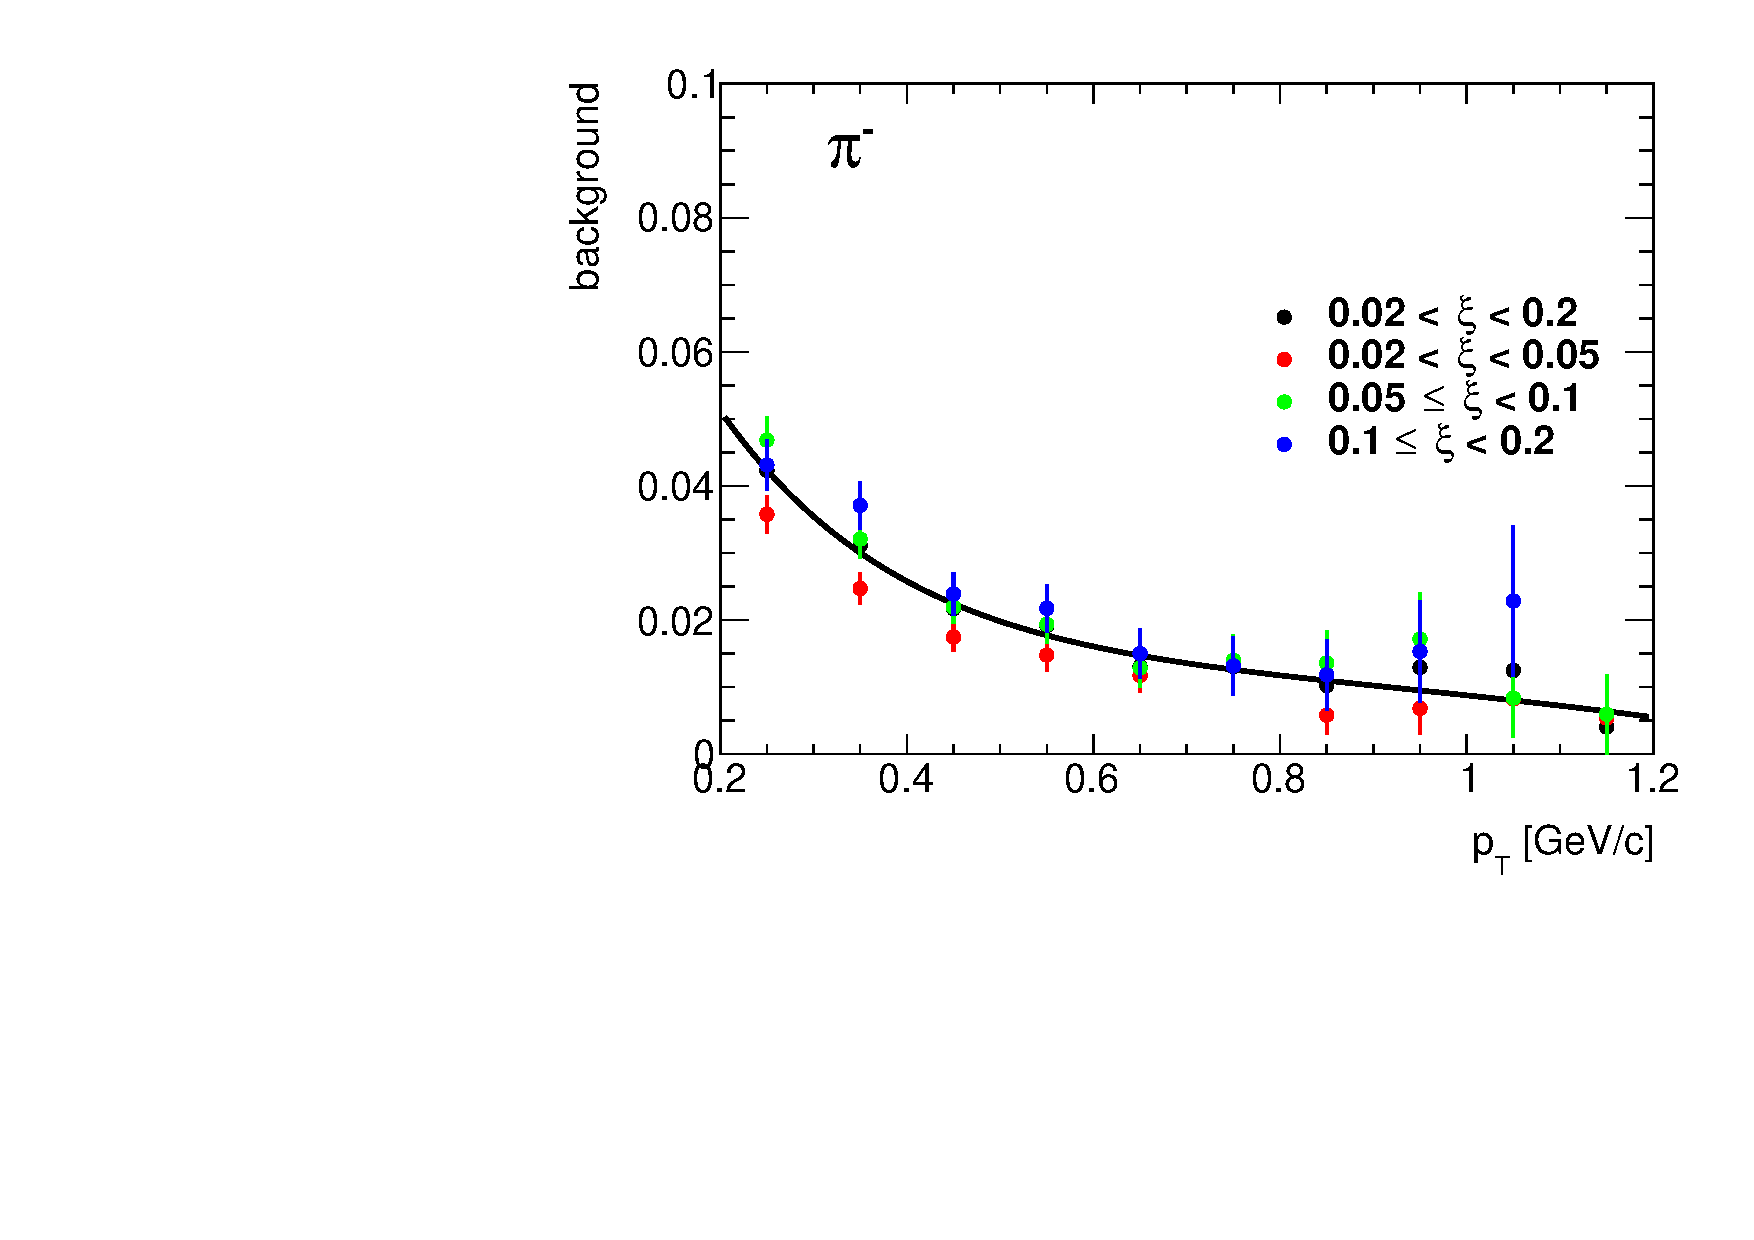
\includegraphics[width=\linewidth, page=1]{chapters/chrgSTAR/img/chargedBkg/bkg0max.pdf}
	\end{subfigure}
	\begin{subfigure}{.49\textwidth}
		\includegraphics[width=\linewidth, page=2]{chapters/chrgSTAR/img/chargedBkg/bkg0max.pdf}
	\end{subfigure}
	\caption{Pion background fraction as a function of $p_\textrm{T}$ calculated from PYTHIA~8 and shown separately for  (left) negatively  and (right)  positively charged pions in three ranges of $\xi$: (red) $0.02<\xi<0.05$,  (green) $0.05<\xi<0.1$, (blue) $0.1<\xi<0.2$.  (full black points) The pion background averaged over three ranges of $\xi$ with fitted parametrization is also shown. Open black points represent EPOS predictions for the full $\xi$ range.}
	\label{fig:bkg_pion}
\end{figure}

\FloatBarrier